\section{Finite Volume Method}

To use the FVM, the solution domain must first be divided into
non-overlapping polyhedral elements or cells.  A solution domain
divided in such a way is generally known as a mesh (as we will see, a
\Class{Mesh} is also a \FiPy{} object).  A mesh consists of vertices,
faces and cells (see Figure~\ref{fig:meshcartoon}).  In the FVM the
variables of interest are averaged over control volumes (CVs).  The
CVs are either defined by the cells or are centered on the vertices.

\begin{figure}
 \begin{center}
%  \resizebox{8cm}{!}{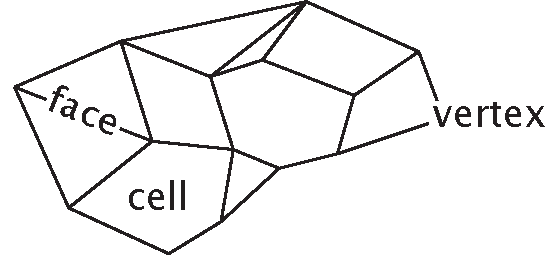
\includegraphics[width=8cm]{numerical/meshcartoon.pdf}}
 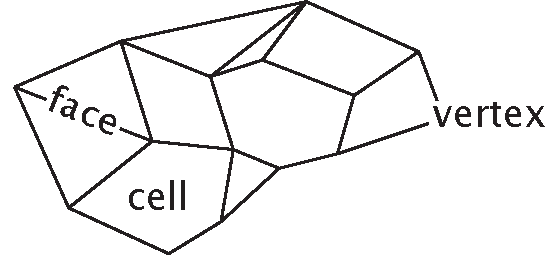
\includegraphics[width=8cm]{numerical/meshcartoon.pdf}
 \caption{A mesh consists of cells, faces and vertices. For the
 purposes of \FiPy{}, the divider between two cells is known as a face
 for all dimensions.}  \label{fig:meshcartoon} \end{center}
\end{figure}

\subsection{Cell Centered FVM (CC-FVM)}

In the CC-FVM the CVs are formed by the mesh cells with the cell
center `storing' the average variable value in the CV, (see
Figure~\ref{fig:vc-cc-fv}). The face fluxes are approximated using the
variable values in the two adjacent cells surrounding the face. This
low order approximation has the advantage of being efficient and
requiring matrices of low band width (the band width is equal to the
number of cell neighbors plus one) and thus low storage
requirement. However, the mesh topology is restricted due to
orthogonality and conjunctionality requirements. The value at a face is
assumed to be the average value over the face. On an unstructured mesh
the face center may not lie on the line joining the CV centers, which
will lead to an error in the face interpolation. \FiPy{} currently
only uses the CC-FVM.

\subsection{Vertex Centered FVM (VC-FVM)}

In the VC-FVM, the CV is centered around the vertices and the cells are
divided into sub-control volumes that make up the main CVs (see
Figure~\ref{fig:vc-cc-fv}).  The vertices `store' the average variable
values over the CVs.  The CV faces are constructed within the cells
rather than using the cell faces as in the CC-FVM. The face fluxes use
all the vertex values from the cell where the face is located to
calculate interpolations.  For this reason, the VC-FVM is less
efficient and requires more storage (a larger matrix band width) than
the CC-FVM. However, the mesh topology does not have the same
restrictions as the CC-FVM. Future releases of \FiPy{} will have both
the CC-FVM and VC-FVM capabilities.

\begin{figure}
\begin{center}
%  \rotatebox{-90}{\resizebox{6cm}{!}{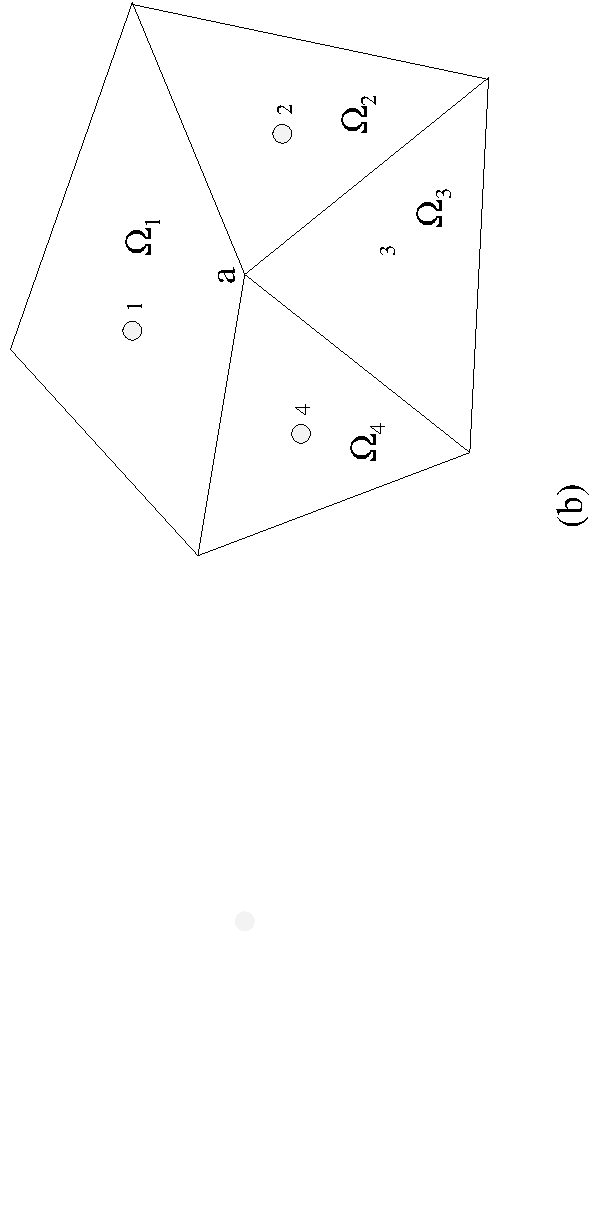
\includegraphics{numerical/vc-cc-fv.pdf}}}
 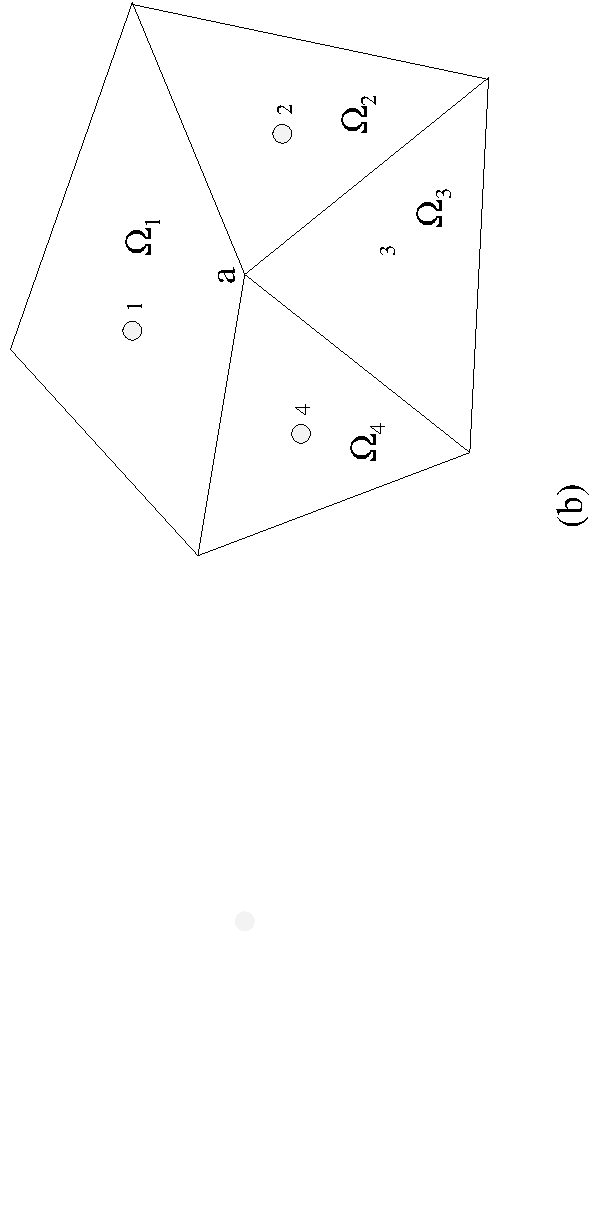
\includegraphics[width=6cm,angle=-90]{numerical/vc-cc-fv.pdf}
 \caption{CV structure for an unstructured mesh, (a) $\Omega_a$
 represents a vertex-based CV and (b) $\Omega_1$, $\Omega_2$,
 $\Omega_3$ and $\Omega_4$ represent cell centered CVs. }
 \label{fig:vc-cc-fv}
\end{center}
\end{figure}

\section{Discretization}

The first step in the discretization of Equation~\eqref{eqn:num:gen}
using the CC-FVM is to integrate over a CV and then make appropriate
approximations for fluxes across the boundary of each CV.  In this
section, each term in Equation~\eqref{eqn:num:gen} will be examined
separately.

\subsection{Transient Term}

For the transient term, the discretization of the integral \( \int_V
\) over the volume of a CV is given by
\begin{equation}
\int_V \frac{\partial (\rho \phi)}{\partial t} dV
\simeq
\frac{(\rho_{P} \phi_{P} - \rho_{P}^\text{old} \phi_{P}^\text{old}) V_P}{\Delta t}
\label{eqn:num:tra}
\end{equation}
where \( \phi_P \) represents the average value of \( \phi \) in a CV
centered on a point \( P \) and the superscript ``$\text{old}$''
represents the previous time-step value.  The value $V_P$ is the
volume of the CV and $\Delta t$ is the time step size.

\subsection{Convection Term}

The discretization for the convection term is given by
\begin{eqnarray}
\int_V \nabla \cdot (\vec{u} \phi)\,dV & = & 
\int_S (\vec{n} \cdot \vec{u})\phi\,dS \\
& \simeq & \sum_{f} (\vec{n} \cdot \vec{u})_f \phi_f A_f
\label{eqn:num:con}
\end{eqnarray}
where we have used the divergence theorem to transform the integral
over the CV volume \( \int_V \) into an integral over the CV surface
\( \int_S \).  The summation over the faces of a CV is denoted by
$\sum_{f}$ and $A_f$ is the area of each face.  The vector $\vec{n}$
is the normal to the face pointing out of the CV into an adjacent CV
centered on point \( A \).  When using a first order approximation,
the value of $\phi_f$ must depend on the average value in adjacent
cell $\phi_A$ and the average value in the cell of interest $\phi_P$,
such that
\begin{equation}
\phi_f=\alpha_f \phi_P +(1-\alpha_f)\phi_A.
\end{equation}
The weighting factor $\alpha_f$ is determined by the convection
scheme, described later in this chapter.

\subsection{Diffusion Term}

The discretization for the diffusion term is given by
\begin{eqnarray}
\int_V \nabla \cdot (\Gamma\nabla\{\ldots\}) dV 
& = & \int_S \Gamma (\vec{n} \cdot \nabla\{\ldots\}) dS \\
& \simeq & \sum_f \Gamma_f (\vec{n} \cdot \nabla\{\ldots\})_f A_f
\label{eqn:num:dif}
\end{eqnarray}
$\{\ldots\}$ indicates recursive application of the specified 
operation on \( \phi \), depending on 
the order of the diffusion term.
The estimation for the flux, $(\vec{n} \cdot \nabla\{\ldots\})_f$, is
obtained via
\begin{equation}
(\vec{n} \cdot \nabla\{\ldots\})_f \simeq \frac{\{\ldots\}_A-\{\ldots\}_P}{d_{AP}}
\end{equation}
where the value of $d_{AP}$ is the distance between neighboring cell
centers.  This estimate relies on the orthogonality of the mesh, and
becomes increasingly inaccurate as the non-orthogonality increases.
Correction terms have been derived to improve this error but are not
currently included in \FiPy{}~\cite{croftphd}.

\subsection{Source Term}

The discretization for the source term is given by, 
\begin{equation}
\int_V S_{\phi}\,dV \simeq S_\phi V_P.
\label{eqn:num:sou}
\end{equation}
Including any negative dependence of $S_\phi$ on $\phi$ increases
solution stability. The dependence can only be included in a linear
manner so Equation~\eqref{eqn:num:sou} becomes
\begin{equation}
V_P (S_0 + S_1 \phi_P),
\end{equation}
where \( S_0 \) is the source which is independent of \( \phi \) and
\( S_1 \) is the coeficient of the source which is linearly dependent
on \( \phi \).

\section{Linear Equations}
\label{section:linear-equations}

The aim of the discretization is to reduce the continuous general
equation to a set of discrete linear equations that can then be solved
to obtain the value of the dependent variable at each CV center. This
results in a sparse linear system that requires an efficient iterative
scheme to solve. The iterative schemes available to \FiPy{} are
currently encapsulated in the \href{#id5}{spmatrix} suite of solvers
and include most common solvers such as the conjugate gradient method
and LU decomposition. There are plans to include other solver suites
that are compatible with \Python{}.

Combining Equations~\eqref{eqn:num:tra}, \eqref{eqn:num:con},
\eqref{eqn:num:dif} and \eqref{eqn:num:sou}, the complete
discretization for equation~\eqref{eqn:num:gen} can now be written for
each CV as
\begin{eqnarray}
\frac{\rho_{P}(\phi_{P} - \phi_P^\text{old}) V_P}{\Delta t}
&=&
\sum_{f} (\vec{n} \cdot \vec{u})_f A_f 
\left[\alpha_f \phi_P +\left(1-\alpha_f\right)\phi_A\right]
\nonumber \\
&&+
\sum_f \Gamma_f A_f \frac{(\phi_A-\phi_P)}{d_{AP}}
+ 
V_P ( S_0 - S_1 \phi_P ).
\label{eqn:num:dis}
\end{eqnarray}

Equation~\eqref{eqn:num:dis} is now in the form of a set of linear
combinations between each CV value and its neighboring values and can be
written in the form
\begin{equation}
a_P \phi_P = \sum_f a_{A} \phi_{A} + b_P,
\label{eqn:num:dap}
\end{equation}
where
\begin{eqnarray}
a_P & = & V_P S_1 + \frac{\rho_P V_P}{\Delta t} + \sum_f (a_{A} -
F_f), \\
a_{A} & = & ( 1 - \alpha_f ) F_f + D_f, \\
b_P & = & V_P S_0 + \frac{\rho_P V_P \phi_P^\text{old}}{\Delta t}.
\end{eqnarray}
The face coefficients, $F_f$ and $D_f$, represent the convective strength
and diffusive conductance respectively, and are given by
\begin{eqnarray}
F_f & = & A_f ( \vec{u} \cdot \vec{n} )_f, \\
D_f & = & \frac{A_f \Gamma_f}{d_{AP}} .
\end{eqnarray}












